\documentclass[tikz]{standalone}
\usepackage{pgfplots}
\pgfplotsset{compat=1.15}
\usepackage{mathrsfs}
\usetikzlibrary{arrows,calc}
\usepackage{tkz-euclide}

\pagestyle{empty}

\definecolor{AngleClr}{rgb}{0,0.39215686274509803,0}
\definecolor{ShapeClr}{rgb}{0.6,0.2,0}
\definecolor{SecondAngleClr}{RGB}{14, 70, 161}

\begin{document}

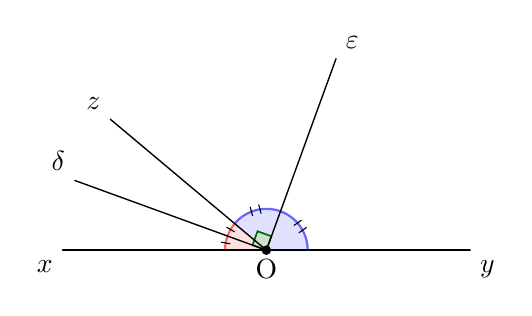
\begin{tikzpicture}[scale=.75]
\tkzSetUpLine[line width=1pt,color=black]
\tkzSetUpPoint[fill=black]

\tkzDefPoints{0/0/O}

\tkzDefPoint(180:3.45){x}
\tkzDefPoint(160:3.45){d}
\tkzDefPoint(140:3.45){z}
\tkzDefPoint(70:3.45){t}
\tkzDefPoint(0:3.45){y}

\tkzFillAngles[fill=red!60!white,size=.7,fill opacity=0.2](d,O,x z,O,d)
\tkzMarkAngles[mark=|,mksize=1.7,line width=0.8pt,size=.7,color=red!60!white](d,O,x z,O,d)

\tkzFillAngles[fill=blue!60!white,size=.7,fill opacity=0.2](t,O,z y,O,t)
\tkzMarkAngles[mark=||,mksize=1.7,line width=0.8pt,size=.7,color=blue!60!white](t,O,z y,O,t)

\tkzMarkRightAngles[line width=0.5pt, size=.25,color=AngleClr,fill=white](t,O,d)
\tkzMarkRightAngles[line width=0.5pt, size=.25,color=AngleClr,fill=AngleClr,fill opacity=0.2](t,O,d)

\tkzDrawSegments[line width=0.5pt,color=black](O,x O,d O,z O,t O,y)


\tkzDrawPoints[size=3](O)
\tkzLabelPoint[below](O){$\rm O$}
\tkzLabelPoint[below left](x){$x$}
\tkzLabelPoint[below right](y){$y$}
\tkzLabelPoint[above left](d){$\delta$}
\tkzLabelPoint[above left](z){$z$}
\tkzLabelPoint[above right](t){$\varepsilon$}

\end{tikzpicture}
\end{document}
